\section{Theorie}\label{sec:theorie}
Nachdem zunächst auf den Grundlegenden Aufbau eines Lasers und die Einzelheiten des Entstehungsprozesses von Laserstrahlung und relevante charakteristische Eigenschaften der Wellen eingegangen wird, folgt mit diesem Wissen eine Einführung in die Funktionsweise des verwendeten \ce{He}-\ce{Ne}-Lasers.
\subsection{Aufbau eines Lasers}
Im wesentlichen besteht ein Laser aus drei Komponenten: dem \textbf{aktiven Medium}, der (selektiven) \textbf{Energiepumpe} und dem \textbf{Resonator}.\\
Das Aktive Medium ist ein Material, welches unter speziellen Vorraussetzungen die Fähigkeit besitzt, die Intensität von durchlaufendem Licht zu verstärken. Dies geschieht, da Atome in solchen Konfigurationen angeregt werden, die induzierte Emission von Photonen wahrscheinlicher als Absorption für bestimmte Frequenzen werden lassen(siehe \hyperref[subsec:entstehung]{Entstehung von Laserstrahlung}).\\
Die Energiepumpe liefert die nötige Energie um die Atome in die gewünschten angeregten Zustände zu heben. Erst durch sie kann der Laserbetrieb ermöglicht werden.\\
Der Resonator, typischerweise bestehend aus zwei Spiegeln, sorgt dafür, dass das Licht mehrmals das aktive Medium durchläuft indem er es hin- und herreflektiert. So kann die Verstärkung der Intensität signifikant genutzt werden, um einen stabilen Strahl zu konstruieren. Diese Energie des Laserstrahls wird zu einem großen Teil im Resonator in wenigen Resonatormoden gespeichert, was zu einer hohen Strahlungsdichte in ausgewählten Wellenlängen führt.\cite{Demtroeder} 
\subsection{Entstehung von Laserstrahlung}\label{subsec:entstehung}
Durch die dem System mittels der Pumpe hinzugeführte Energie werden die Atome des aktiven Mediums von ihrem Grundzustand in verschiedene höher gelegene Energieniveaus gehoben.
Sei etwa $k$ ein energetisch höherer quantenmechanischer Zustand des Atoms als ein mit ihm durch einen erlaubten Übergang verbundener Zustand $i$, so würde im thermischen Gleichgewicht für die Besetzungszahlen der Zustände $N_i>N_k$ gelten. Die erwähnte selektive Energiezufuhr führt nun dazu, dass wie in \autoref{fig:inversion} dargestellt, sich die Besetzungsverteilung verändert, es tritt \textbf{Besetzungsinversion} auf.
\begin{figure}[H]
    \centering
    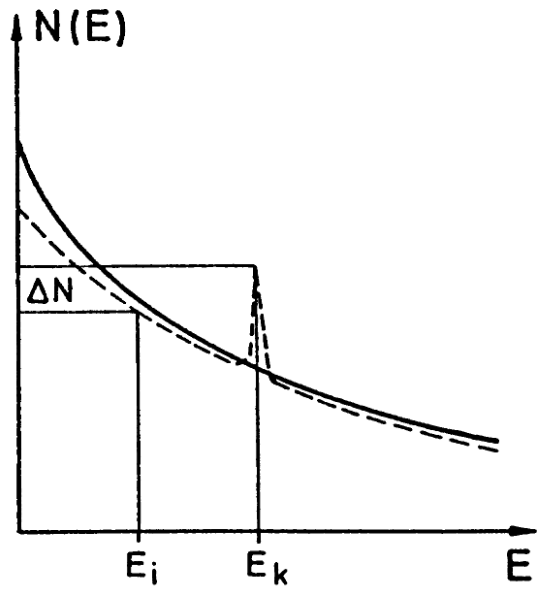
\includegraphics[scale=0.5]{Ressourcen/inversion.png}
    \caption{Thermische Besetzungsverteilung (durchgezogen) und Inversion (gestrichelt)\cite{Demtroeder}}\label{fig:inversion}
\end{figure}
Trifft ein Photon der Frequenz $\nu = \frac{E_k-E_i}{h}$ auf ein angeregtes Atom oder Molekül der Energie $E_k$, so kann es dieses dazu veranlassen in den tieferen Zustand $E_i$ überzugehen unter Emission eines Photons derselben Frequenz und Richtung.

\subsection{Eigenschaften von Laserstrahlung}
\subsection{Funktionsweise eines He-NeLasers}